\documentclass[letter,11pt]{article}

\usepackage[spanish,es-nodecimaldot]{babel}
\usepackage[utf8]{inputenc}

\usepackage{lmodern}
\usepackage[T1]{fontenc}
\usepackage{textcomp}

\usepackage{framed}
\usepackage[svgnames]{xcolor}
\colorlet{shadecolor}{Gainsboro!50}

\usepackage[shortlabels]{enumitem}
\usepackage{graphicx}
\usepackage{pstricks}

\usepackage{anysize}
\marginsize{3cm}{2cm}{2cm}{3cm}

\usepackage{siunitx}
\usepackage{amsmath}
\usepackage{amssymb}
\usepackage{array}

\usepackage{fancyhdr}
\usepackage{lastpage}
\pagestyle{fancy}
\fancyhf{}
\fancyhead[LE,RO]{Física Básica II}
\fancyfoot[CO,CE]{\thepage\ de \pageref{LastPage}}

\special{papersize=215.9mm,279.4mm}

\usepackage[
    pdfauthor={Carlos Eduardo Caballero Burgoa},%
    pdftitle={Física Básica II},%
    pdfsubject={Tarea 25},%
    colorlinks,%
    citecolor=black,%
    filecolor=black,%
    linkcolor=black,%
    urlcolor=black,
    breaklinks]{hyperref}
\usepackage{breakurl}

\newcommand{\blankpage}{
\newpage
\thispagestyle{empty}
\mbox{}
\newpage
}

\renewcommand{\arraystretch}{1.2}

\begin{document}

\begin{center}
    {\Large \bf{Tarea \#25}}
\end{center}

1) Demostrar y/o verificar las ecuaciones:

\begin{enumerate}[a)]
    \item \underline{Caso I}: Movimiento aperiódico sobre-amortiguado
        \begin{equation*}
            \begin{cases}
                x_0 = A_1 + A_2 \\
                \dot{x}_0 = (\omega_{sa} - b) A_1 - (\omega_{sa} + b) A_2
            \end{cases}
        \end{equation*}
        \begin{equation*}
            \therefore\,
            \begin{cases}
                A_1 = \dfrac{(\omega_{sa} + b) x_0 + \dot{x}_0}{2\omega_{sa}} \\
                \\
                A_2 = \dfrac{(\omega_{sa} - b) x_0 - \dot{x}_0}{2\omega_{sa}}
            \end{cases}
        \end{equation*}
        \vspace{0.1cm}
    \item \underline{Caso II}: Movimiento aperiódico crítico
        \begin{equation*}
            \begin{cases}
                x_0 = A_1 \\
                \dot{x}_0 = A_2 - A_1 b
            \end{cases}
        \end{equation*}
        \begin{equation*}
            \therefore\,
            \begin{cases}
                A_1 = x_0 \\
                A_2 = \dot{x}_0 + x_0 b
            \end{cases}
        \end{equation*}
        \vspace{0.1cm}
    \item \underline{Caso III}: Movimiento oscilatorio amortiguado
        \begin{equation*}
            \begin{cases}
                x_0 = R\,cos(\theta) \\
                \dot{x}_0 = -R\,(b\,cos(\theta)-\omega'\,sin(\theta))
            \end{cases}
        \end{equation*}
        \begin{equation*}
            \therefore\,
            \begin{cases}
                R = \dfrac{\sqrt{(\omega'x_0)^2+(\dot{x}_0+b\,x_0)^2}}{\omega'} \\
                \\
                cos(\theta) = \dfrac{\omega'x_0}{\sqrt{(\omega'x_0)^2+(\dot{x}_0+b\,x_0)^2}}
            \end{cases}
        \end{equation*}
\end{enumerate}

\vspace{0.5cm}
\textbf{Solución:} \\

\textbf{(a)} \\

Considerando el sistema de 2 ecuaciones lineales con 2 incógnitas:

\begin{equation*}
    \begin{cases}
        A_1 + A_2 = x_0 \\
        (\omega_{sa} - b) A_1 - (\omega_{sa} + b) A_2 = \dot{x}_0
    \end{cases}
\end{equation*}
\\

Y resolviendo por el método de determinantes, obtenemos:

\begin{equation}
    A_1 = \dfrac{
        \left|
            \begin{smallmatrix}
                x_0 & 1 \\
                \dot{x}_0 & -(\omega_{sa} + b)
            \end{smallmatrix}
        \right|
    }{
        \left|
            \begin{smallmatrix}
                1 & 1 \\
                (\omega_{sa} - b) & -(\omega_{sa} + b)
            \end{smallmatrix}
        \right|
    }
    = \dfrac{-x_0 \omega_{sa} - x_0 b - \dot{x}_0}{-\omega_{sa} - b - \omega_{sa} + b}
    = \dfrac{-(\omega_{sa} + b) x_0 - \dot{x}_0}{-2\omega_{sa}}
    = \dfrac{(\omega_{sa} + b) x_0 + \dot{x}_0}{2\omega_{sa}}
\end{equation}

\begin{equation}
    A_2 = \dfrac{
        \left|
            \begin{smallmatrix}
                1 & x_0 \\
                (\omega_{sa} - b) & \dot{x}_0
            \end{smallmatrix}
        \right|
    }{
        \left|
            \begin{smallmatrix}
                1 & 1 \\
                (\omega_{sa} - b) & -(\omega_{sa} + b)
            \end{smallmatrix}
        \right|
    }
    = \dfrac{\dot{x}_0 - x_0\omega_{sa} + x_0 b}{-\omega_{sa} - b - \omega_{sa} + b}
    = \dfrac{-(\omega_{sa} - b) x_0 + \dot{x}_0}{-2\omega_{sa}}
    = \dfrac{(\omega_{sa} - b) x_0 - \dot{x}_0}{2\omega_{sa}}
\end{equation}
\\

\textbf{(b)} \\

Considerando el sistema de 2 ecuaciones lineales con 2 incógnitas:

\begin{equation*}
    \begin{cases}
        A_1 = x_0 \\
        A_1 b - A_2 = -\dot{x}_0
    \end{cases}
\end{equation*}
\\

Y resolviendo por el método de determinantes, obtenemos:

\begin{equation}
    A_1 = \dfrac{
        \left|
            \begin{smallmatrix}
                x_0 & 0 \\
                -\dot{x}_0 & -1
            \end{smallmatrix}
        \right|
    }{
        \left|
            \begin{smallmatrix}
                1 & 0 \\
                b & -1
            \end{smallmatrix}
        \right|
    }
    = \dfrac{-x_0}{-1}
    = x_0
\end{equation}

\begin{equation}
    A_2 = \dfrac{
        \left|
            \begin{smallmatrix}
                1 & x_0 \\
                b & -\dot{x}_0
            \end{smallmatrix}
        \right|
    }{
        \left|
            \begin{smallmatrix}
                1 & 0 \\
                b & -1
            \end{smallmatrix}
        \right|
    }
    = \dfrac{-\dot{x}_0 - x_0 b}{-1}
    = \dot{x}_0 + x_0 b
\end{equation}
\\

\textbf{(c)} \\

Considerando el sistema de 2 ecuaciones con 2 incógnitas:

\begin{equation*}
    \begin{cases}
        x_0 = R\,cos(\theta) \\
        \dot{x}_0 = -R\,(b\,cos(\theta)-\omega'\,sin(\theta))
    \end{cases}
\end{equation*}
\\

Despejando $R$ de la primera ecuación:

\begin{equation*}
    R = \frac{x_0}{cos(\theta)}
\end{equation*}
\\

Y reemplazando en la segunda ecuación:

\begin{equation*}
    \dot{x}_0 = -R\,b\,cos (\theta) + R\,\omega'\,sen(\theta)
\end{equation*}
\begin{equation*}
    \dot{x}_0 = - \frac{x_0}{cos(\theta)}\,b\,cos (\theta) + \frac{x_0}{cos(\theta)}\,\omega'\,sen(\theta)
\end{equation*}
\begin{equation*}
    \dot{x}_0 = - x_0\,b + x_0\,\omega'\,\frac{sen(\theta)}{cos(\theta)}
\end{equation*}
\begin{equation*}
    \frac{\dot{x}_0 + x_0\,b}{x_0\,\omega'} = tan(\theta)
\end{equation*}
\\

Considerando el valor de la tangente de $\theta$, podemos formar el siguiente
triangulo rectángulo:

\begin{figure}[!h]
\centering
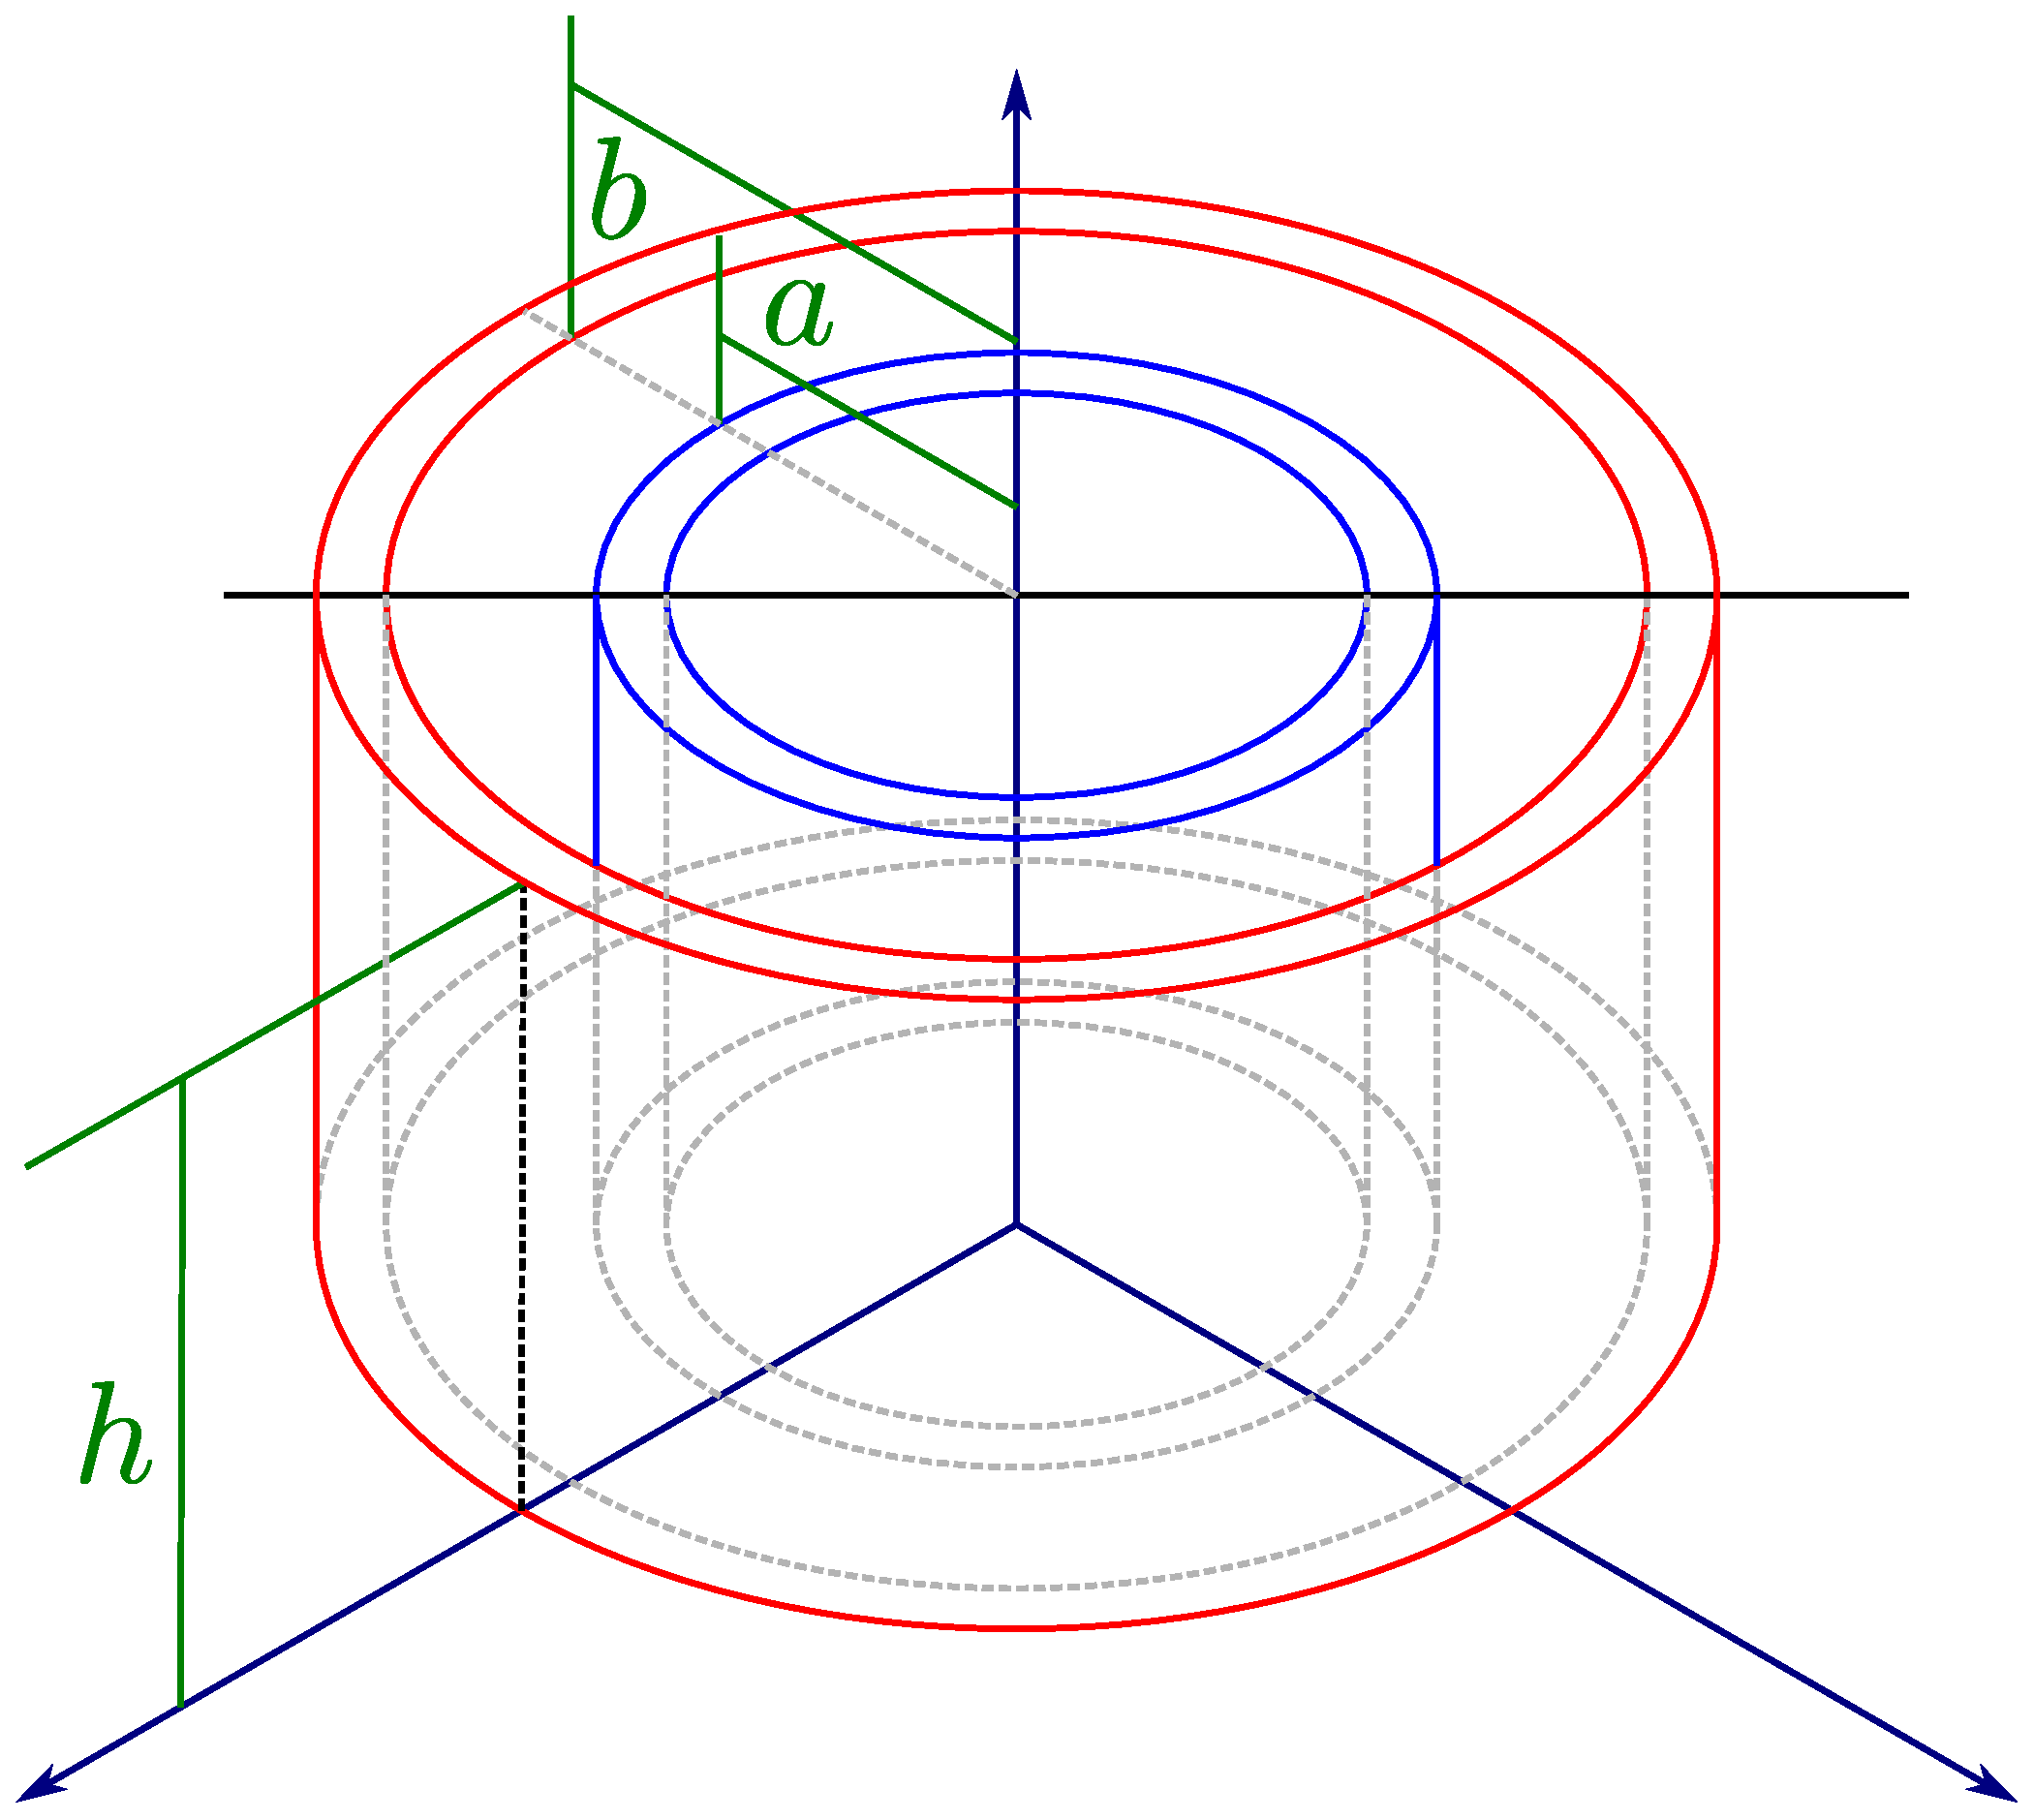
\includegraphics[scale=0.40]{resources/f1.eps}
\end{figure}

Cuyo valor de la hipotenusa es:

\begin{equation*}
    h^2 = (x_0\,\omega')^2 + (\dot{x}_0 + x_0\,b)^2
\end{equation*}
\begin{equation*}
    h = \sqrt{ (x_0\,\omega')^2 + (\dot{x}_0 + x_0\,b)^2 }
\end{equation*}
\\

Por tanto, es posible calcular el valor del coseno:

\begin{equation}
    cos(\theta) = \frac{x_0\omega'}{\sqrt{ (x_0\,\omega')^2 + (\dot{x}_0 + x_0\,b)^2 }}
\end{equation}
\\

Despejando $R$ de la primera ecuación, obtenemos:

\begin{equation*}
    R = \frac{x_0}{cos(\theta)}
\end{equation*}
\begin{equation*}
    R = x_0\,\frac{\sqrt{ (x_0\,\omega')^2 + (\dot{x}_0 + x_0\,b)^2 }}{x_0\omega'}
\end{equation*}
\begin{equation}
    R = \frac{\sqrt{ (x_0\,\omega')^2 + (\dot{x}_0 + x_0\,b)^2 }}{\omega'}
\end{equation}

\vspace{1.0cm}
2) Una partícula de masa $1\,[g]$ se mueve a lo largo del eje $x$ bajo la
influencia de dos fuerzas: $(i)$ una fuerza de atracción hacia el origen que es
numéricamente igual a $4x\,[dinas]$, y $(ii)$ una fuerza de amortiguación cuya
magnitud en $dinas$ es numéricamente igual a $6$ veces la velocidad instantánea.
Suponiendo que la partícula comienza desde el reposo a una distancia de
$10\,[cm]$ del origen.

\begin{enumerate}[a)]
    \item Establezca la ecuación diferencial del movimiento de la partícula.
    \item Encuentre la posición de la partícula en cualquier momento.
    \item Determine la amplitud, periodo y frecuencia de la oscilación
        amortiguada.
\end{enumerate}

\vspace{0.5cm}
\textbf{Solución:} \\

\begin{figure}[!h]
\centering
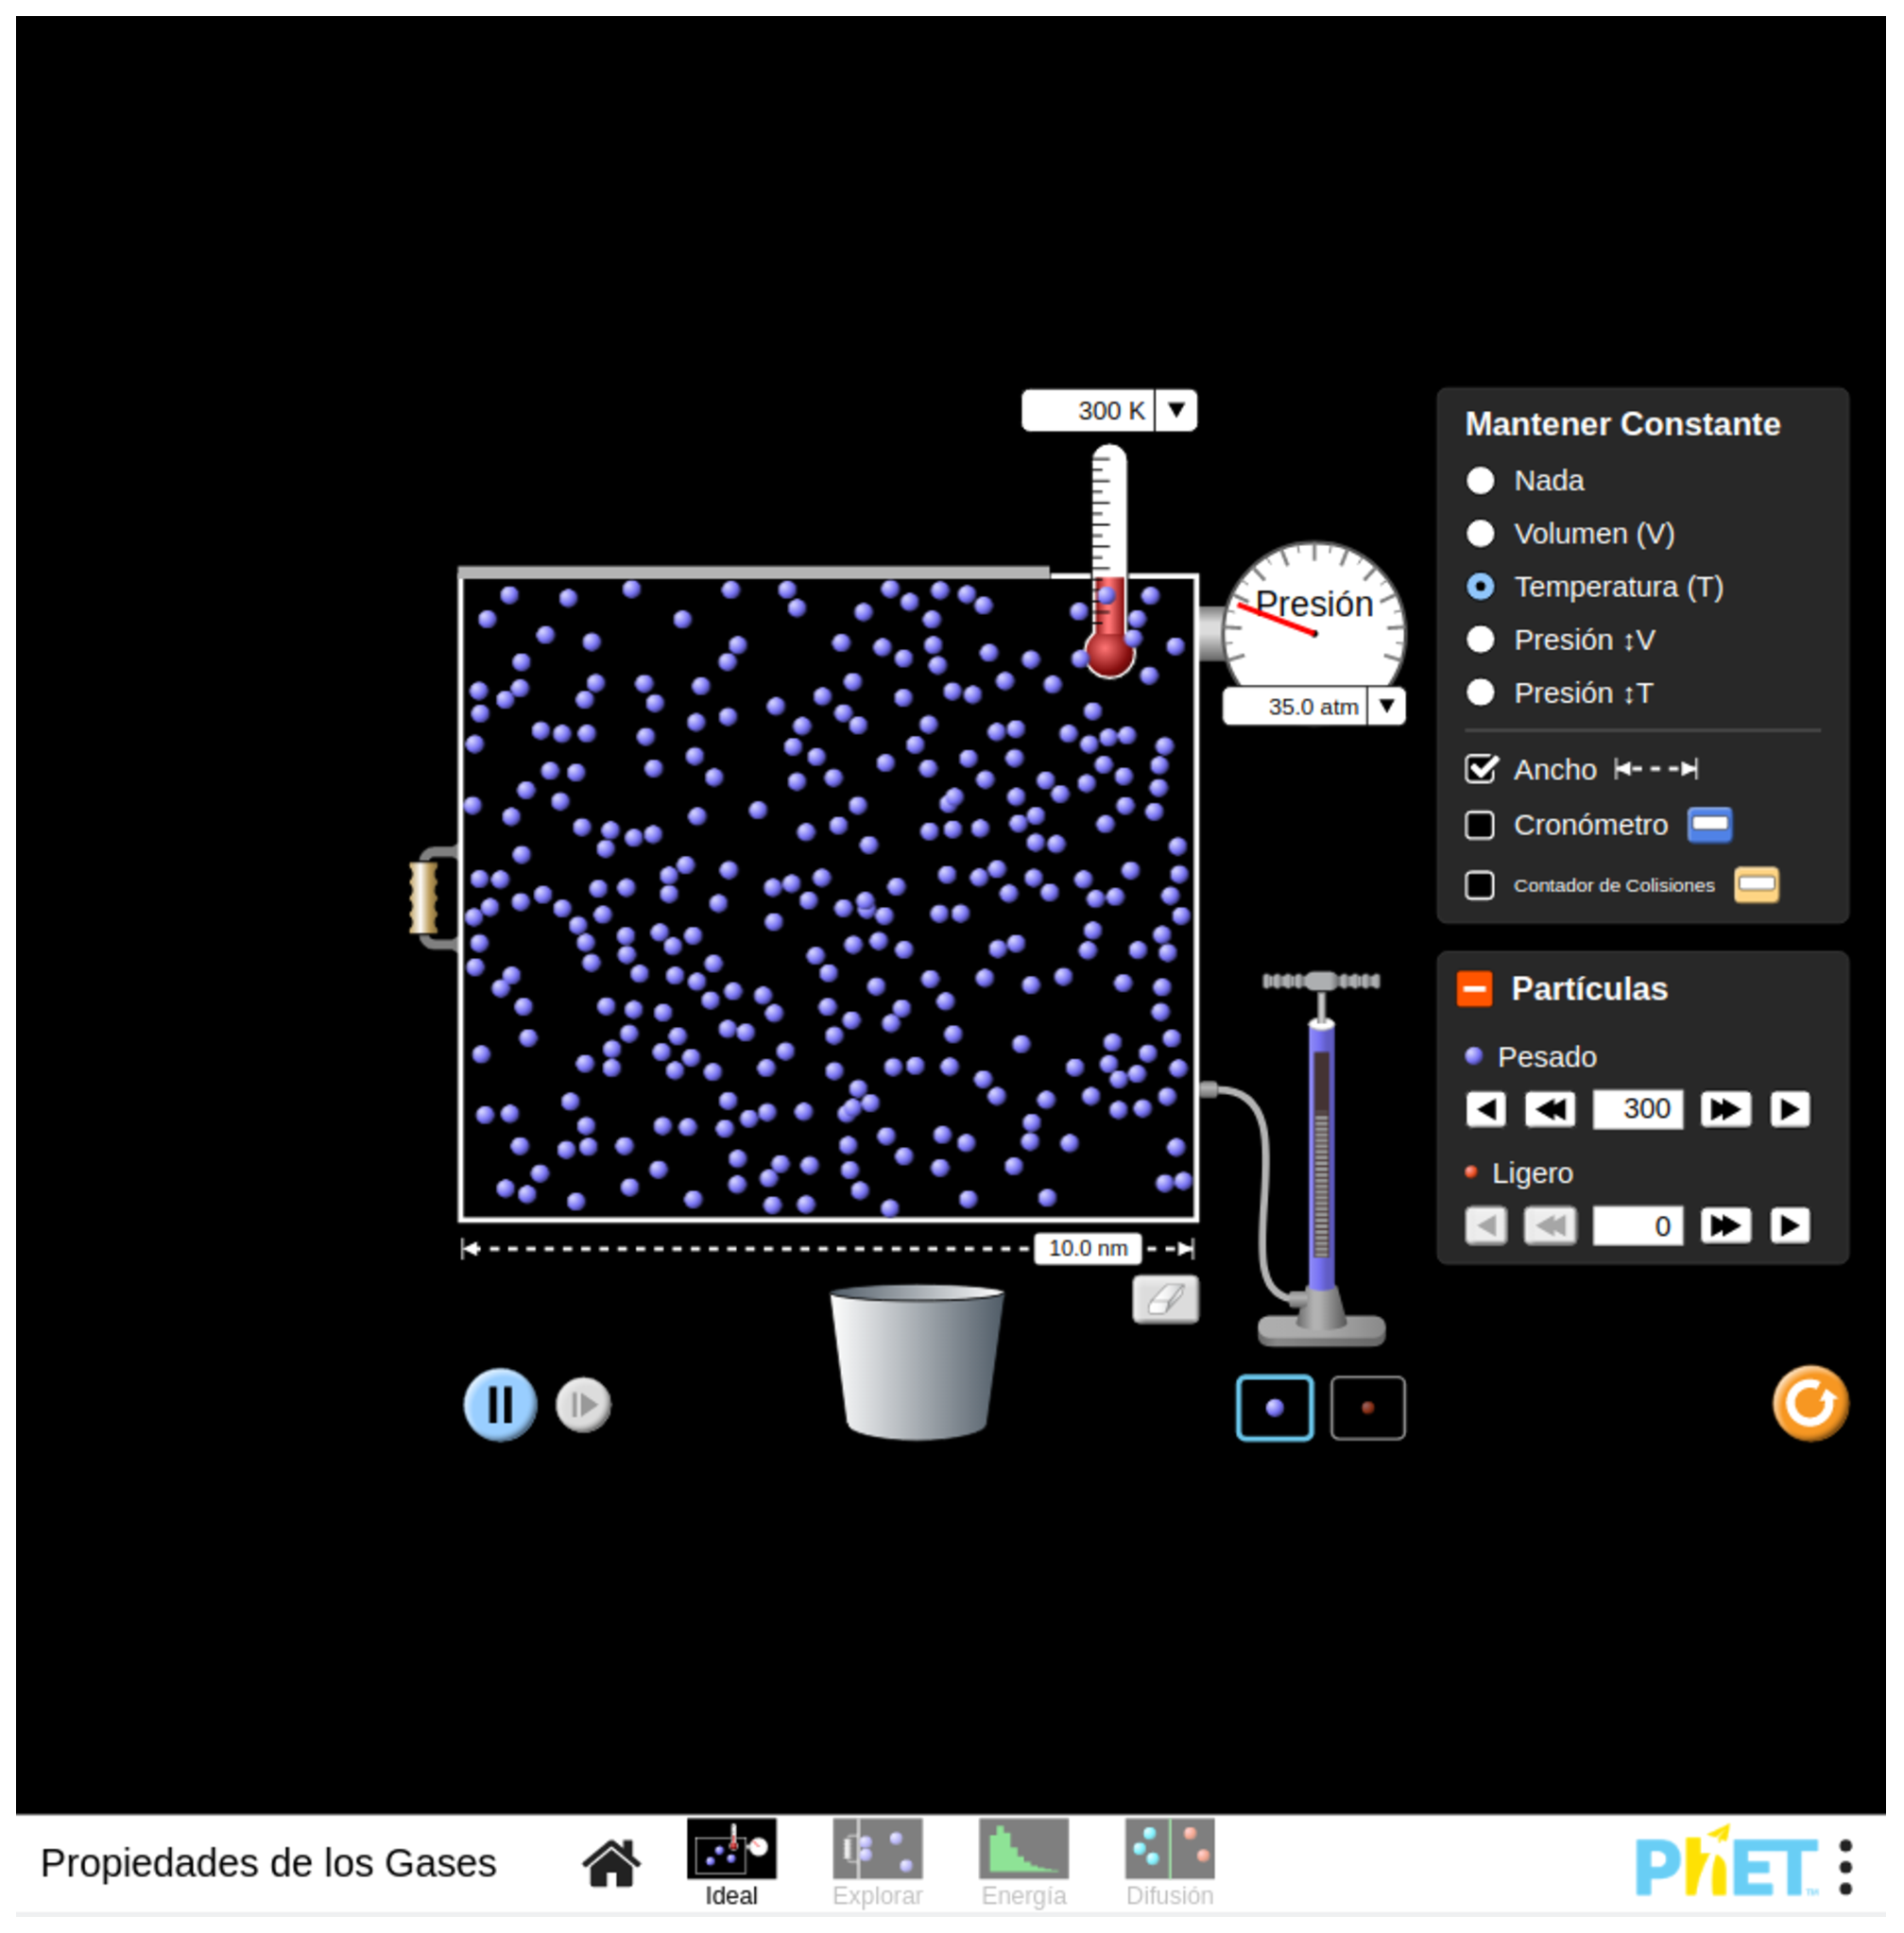
\includegraphics[scale=0.40]{resources/f2.eps}
\end{figure}

\textbf{(a)} \\

Considerando la segunda ley de \emph{Newton}:

\begin{equation*}
    \sum F = m\, a
\end{equation*}
\begin{equation*}
    - F - F_a = m\, a
\end{equation*}
\begin{equation*}
    - 4x - 6\dot{x} = 1\, \ddot{x}
\end{equation*}

Por tanto:

\begin{equation}
    \ddot{x} + 6 \dot{x} + 4 x = 0
\end{equation}

\textbf{(b)} \\

Comparando con la ecuación diferencial de un oscilador armónico amortiguado:

\begin{equation*}
    \ddot{x} + 2b\dot{x} + \omega^2_0x=0
\end{equation*}

Se obtienen el valor de $b$ y $\omega_0$:

\begin{equation*}
    2b = 6
\end{equation*}
\begin{equation}
    b = 3
\end{equation}

\begin{equation*}
    \omega^2_0 = 4
\end{equation*}
\begin{equation}
    \omega_0 = 2
\end{equation}

Al ser $b > \omega_0$, se considera un movimiento aperiódico sobre-amortiguado
(Caso I).

Por tanto:

\begin{equation*}
    \omega_{sa} = \sqrt{b^2-\omega^2_0} = \sqrt{3^2-2^2} = \sqrt{5}
\end{equation*}
\begin{equation*}
    A_1 = \dfrac{(\omega_{sa} + b) x_0 + \dot{x}_0}{2\omega_{sa}} = \frac{(\sqrt{5} + 3) 10 + 0}{2\sqrt{5}} = 11.708
\end{equation*}
\begin{equation*}
    A_2 = \dfrac{(\omega_{sa} - b) x_0 - \dot{x}_0}{2\omega_{sa}} = \frac{(\sqrt{5} - 3) 10 - 0}{2\sqrt{5}} = -1.708
\end{equation*}

Resultando la ecuación de $x(t)$:

\begin{equation*}
    x(t) = e^{-bt} \left( A_1 e^{\sqrt{b^2-\omega^2_0}t} + A_2 e^{-\sqrt{b^2-\omega^2_0}t} \right)
\end{equation*}
\begin{equation*}
    x(t) = e^{-3t} \left( 11.708 e^{\sqrt{5}t} - 1.708 e^{-\sqrt{5}t} \right)
\end{equation*}
\begin{equation*}
    x(t) = 11.708 e^{(-3 + \sqrt{5})t} - 1.708 e^{(-3 -\sqrt{5})t}
\end{equation*}
\begin{equation}
    x(t) = 11.708 e^{-0.7639t} - 1.708 e^{-5.2361t}\,[cm]
\end{equation}

\textbf{(c)} \\

Considerando que es un movimiento aperiódico sobre-amortiguado, esta carece de
los parámetros $\omega'$, $T$ y $f$.

\end{document}
